\documentclass[letterpaper,10pt]{article}
\usepackage[T1]{fontenc}
\usepackage[utf8]{inputenc}
\usepackage{lmodern}
\usepackage{amsmath}
\usepackage{cancel}
\usepackage[margin=1.5in]{geometry}
\usepackage{verbatim}
\usepackage{scrextend}
\usepackage{longtable}
\usepackage{framed}
\usepackage{amssymb}
\usepackage{wasysym}
\usepackage{multicol}
\usepackage{graphicx}
\usepackage{color}
\usepackage{caption}
\usepackage{subcaption}
\usepackage{float}
\usepackage{fancyhdr}
\usepackage[utf8]{inputenc}
\usepackage[mathletters]{ucs}
\usepackage{hyperref}
\usepackage{tikz,tkz-euclide}
\usepackage{pstricks,pst-plot,pst-node,pstricks-add}

\hypersetup
{
  colorlinks=false,
	pdfborder={0 0 0}
}


\pagestyle{fancy}
\lhead{Joseph Mate - jmate - 20246021}
\rhead{CS 648 - Professor Ilyas - UI Optimizer}
\DeclareRobustCommand\iff{\;\Longleftrightarrow\;}

\begin{document}

\raggedright

\setlength{\columnseprule}{0.5pt}


\section{Introduction}
The Postgres query planner does not necessarily return the best plan even with
interesting orders. As mentioned in the CORDS paper, one reason is the estimated
numbers of rows returned by a scan or join can be way off \cite{Ilyas04}. For
instance, imagine the estimate claiming that one row is returned from both
relations in a join. The optimizer might estimate one row because of the
indepedence assumption of AND clauses. The optimizer might perform a nested loop
join because the single row fits in memory. \\[0.5cm]

As a result, this prototype was created to explore the possibility of a
database user manually manipulating the plan, or changing the estimates of
the number rows returned from a base or joined relation. The primary use case is
for queries that are expected to take hours or days to complete. If used in
other settings, then the time spent having the user optimizing the query may
exceed the time saved in query processing.

\section{Features}
The prototype begins by displaying the plan that the optimizer initially
computes. The UI can display any number of levels of joins. From that UI, you
can change which join algorithm should be applied on two relations. Lastly, the
UI also allows you to modify the the estimated number of rows for each relation
and then the query planner searches for a new plan using the new estimates.

\section{How it Works}
Here I provided a summary of the most complicated components of this project. A
lot of challenges I encountered are not included here to keep the report brief.

\subsection{UI}
The UI was built using GTK+. The most complicated component is the display of
tree. This was solved using a table like GUI abstraction, which a GUI widget can
be placed at any row and column of the table. The follow diagram illustrates how
the formula was derived.

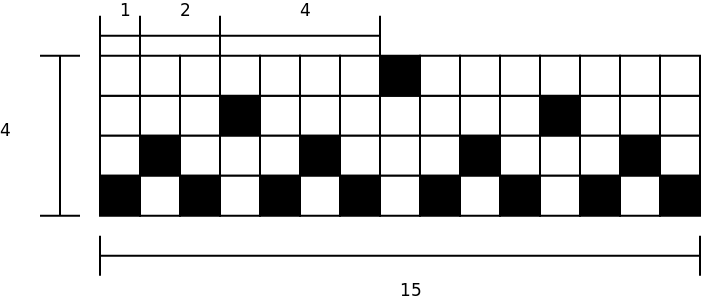
\includegraphics[scale=0.5]{table-derivation.png}

The 0th row is the top most row of the table. The 0th column is the left most
column of the table. Given the above convetion, we can compute the position of
all the nodes using the following recursive formulae \\
\begin{align*}
	row_{root} & = 0 \\
	colum_{root} & = 2^{TreeHeight-1}-1 \\
	row_{child} & = row_{parent} + 1 & \mbox { for both left and right children}\\
	column_{child} & = column_{parent} - 2^{height_{parent}-2} & \mbox { for the left child} \\
	column_{child} & = column_{parent} + 2^{height_{parent}-2} & \mbox { for the right child} \\
\end{align*}

The number of rows is the height of the plan. The child node of a parent, is 1
row below the parent. Additionally, it is $2^{ParentHeight-2}$ units to the left
or the right of the parent.

\subsection{Changing Joins}
The prototype wraps the plan tree datastructure returned by query planner inside
its own tree so that each node of the tree has pointers to any important GUI
widgets that the user may have manipulated. When the user changes the join on
the GUI, we recursively rebuild the path upwards starting from the node that was
changed. This updates the costs all the way up. The user can selects one of the
joins populated in the drop down list and hits the change button. A screenshot
is provided below.

\begin{center}
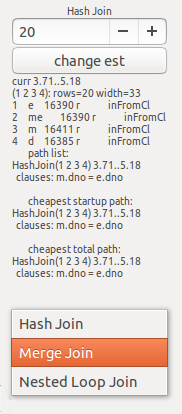
\includegraphics[scale=0.5]{join-ddl.png}
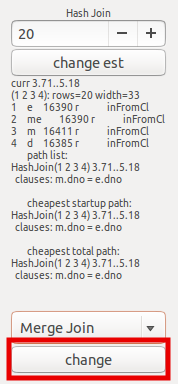
\includegraphics[scale=0.5]{join-ddl-selected.png}
\end{center}

\subsection{Changing a Relation's Rows Estimates}
The prototype adds a hashtable to the PlannerInfo struct. The hashtable is a map
from relids belonging to the relation accumulated so far in the tree to the
overridden estimated number of rows. If the hashtable does not contain an entry
for a given relids, then the estimate for that relation has not been overridden.
Whereever the estimated number of rows was accessed in costsize.c, a lookup to
the hashtable to check if it has been overridden prepended. Additionally, the
follow functions also check for overridden estimates:
\textit{set\_baserel\_size\_estimates, set\_joinrel\_size\_estimates, and
get\_parameterized\_joinrel\_size}. Lastly, the user changes the estimated number of
rows by changing the textbox provided inside the GUI widget representing that
relation and then hits . A screenshot below is provided for reference.

\begin{center}
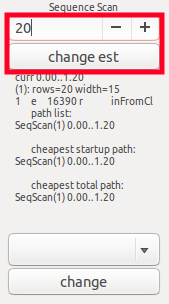
\includegraphics[scale=0.5]{change-estimate.png}
\end{center}



\section{Future Work}
Firstly, in order to focus on the functionality of this prototype, the GUI runs
on the database process, This avoided having to implement a communication
protocol between the database and client and figuring out how to serialize that
data. Secondly, currently there is no way to maniupate the structure of the
tree. Thirdly, there is no way to change which scan should be performed on a
based relation. Fourthly, only one pathkey is considered for the merge join. A
variety of options should be presented to the user selecting merge join. Lastly,
there is absolutely no validation to assist the user when he creates something
that does not make sense.

\section{Acknowledgements}
I would like to thank José Calvo for recommending that I place the GUI directly
on the database server so that I would not have to figure out how to serialize
data between the server and client.

\nocite{*}               
\bibliographystyle{plain}
\bibliography{write-up}     


\end{document}
